\begin{figure*}[t]
\centering
\begin{subfigure}[htb!]{0.3\textwidth}
    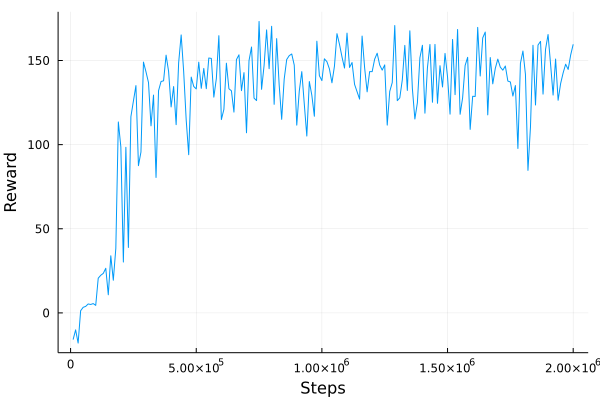
\includegraphics[width=\textwidth]{images/Reward_slow.png}
    \caption{Reward per step for the slow learning phase in 2D.}
    \label{fig:reward_slow}
\end{subfigure}
\hfill
\begin{subfigure}[htb!]{0.3\textwidth}
    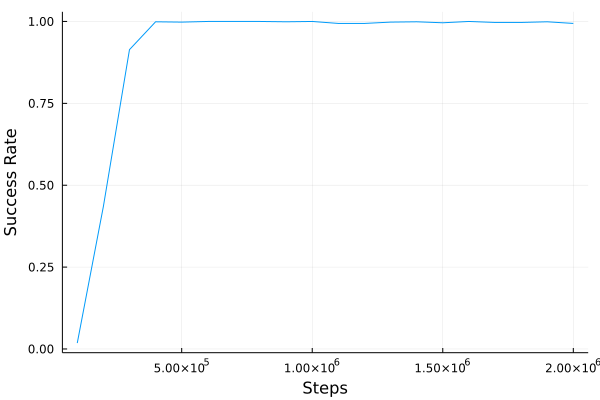
\includegraphics[width=\textwidth]{images/Success_slow.png}
    \caption{Success rate per step for the slow learning phase in 2D.}
    \label{fig:success_slow}
\end{subfigure}
\hfill
\begin{subfigure}[htb!]{0.3\textwidth}
    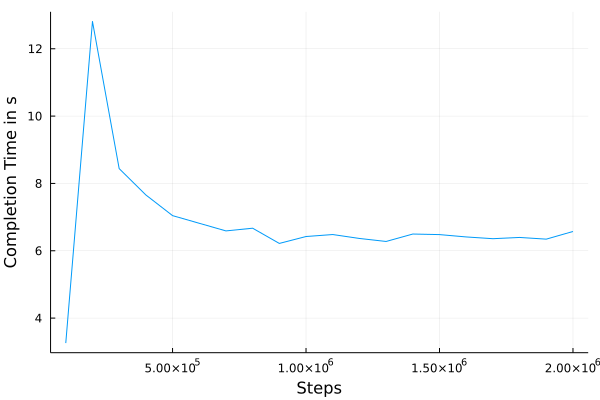
\includegraphics[width=\textwidth]{images/Time_slow.png}
    \caption{Completion time of successful attempts per step for the slow learning phase in 2D.}
    \label{fig:time_slow}
\end{subfigure}
\caption{Experimental setup described in Section \ref{sec:experiments}. Note that in \ref{fig:time_slow} the completion time in step 1 is set to zero, since there were no successful flights.}
\label{fig:results}
\end{figure*}
All the experiments were executed inside the Flyonic's physic simulation environment \cite{flyonic}. 
For the scope of our group's milestone report, we reduced our experiments to a 2D plane (xz-plane). We have disabled all forces that would conflict with this 2D-world, as well as the possible actions regarding the flaps of the drone. It is noteworthy that the gravity is still enabled, having an orientation antiparallel to the z-axis.
\par
The drone is trained for a total of two million time steps with a step size of $\Delta t$. 
In each episode a trajectory with 4 waypoints (including the starting point in the origin) is generated as follows:
The derivation from the previous point is randomly sampled from the uniform distributions $\mathcal{U}(-7, +7)$ for the x-axis and $\mathcal{U}(+1.5, +7)$ for the z-axis. Then, the guiding trajectory is given by the three straight lines connecting the waypoints. 
\par
A flight is considered a success, if each of the four points is passed within a tolerance of $r_{tol}$. This is also reflected through the chosen termination criteria. An episode terminates once one of the following conditions is met:
\begin{itemize}
    \item Drone falls 5 meters below the initial level
    \item Episode takes longer than $10.0 \cdot n$ seconds
    \item Drone deviates more than 5 meter from trajectory
    \item All waypoints were reached
\end{itemize}
\par
During training, every 100,000 steps the current state of the model is saved for further evaluation, which is topic of Section \ref{results}.